\section{Das Buffonsche Nadelproblem}

In diesem Kapitel werden wir nun das Buffonsche Nadelproblem genauer betrachten. Im Jahre 1733 stellte sich Buffon folgende Frage:\\
\textit{Mit welcher Wahrscheinlichkeit schneidet eine willk"urlich geworfene Nadel ein Gitter paralleler Linien?}\\

\underline{\textbf{Probleml"osung bzw. experimentelle Durchf"uhrung:}}\\[0,2cm]

Ben"otigt werden m"oglichst viele identische Nadeln gleicher L"ange $l$. Auf einer Ebene werden parallele Linien mit einem bestimmen Abstand $d$ konstruiert. Die Nadeln werden anschlie"send auf diese Ebene geworfen und es wird gez"ahlt, wie viele dieser geworfenen Nadeln eine Linie kreuzen.\\ Man stellt fest, dass man dadurch eine Ann"aherung der Zahl $\pi$ bekommt.\\
Wir betrachten in unserem Problem Nadeln der L"ange $\lambda \in [0,1]$, die nacheinander auf eine Ebene mit Linien mit Abstand $1$ geworfen werden.  Um eine Antwort auf obige Frage zu erhalten, f"uhren wir folgende Menge  $\Omega=[0,\frac{1}{2}]\times [0,\frac{\pi}{2}] $ ein.\\
Dabei repr"asentiert bei $(x,\alpha)\in \Omega$ die erste Komponente $x$ den Abstand vom Mittelpunkt der Nadel zur n"achsten parallelen Linie in der Ebene. Die zweite Komponente $\alpha$ beschreibt den Winkel, der von der Nadel und der getroffenen Linie eingeschlossen wird.

\begin{figure} [H]
\centering
    \subfigure[Nadeln auf Ebene]{
		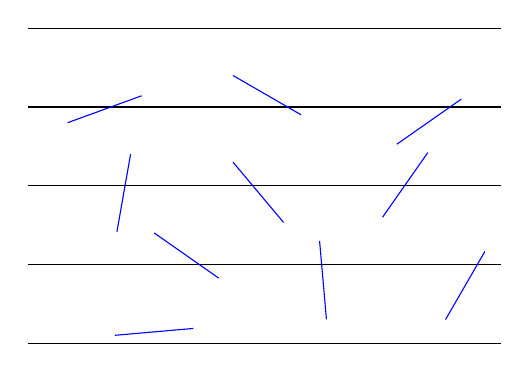
\begin{tikzpicture}
		\draw (0,0) -- (6,0);
		\draw (0,1) -- (6,1);
		\draw (0,2) -- (6,2);
		\draw (0,3) -- (6,3);
		\draw (0,4) -- (6,4);

\draw [blue](0.5,2.8) -- +(20:1cm);
\draw [blue](2.6,3.4) -- +(-30:1cm);
\draw [blue](5.5,3.1) -- +(215:1cm);

\draw [blue](1.3,2.4) -- +(260:1cm);
\draw [blue](2.6,2.3) -- +(310:1cm);
\draw [blue](4.5,1.6) -- +(55:1cm);

\draw [blue](1.6,1.4) -- +(-35:1cm);
\draw [blue](3.7,1.3) -- +(-85:1cm);

\draw [blue](1.1,0.1) -- +(5:1cm); 
\draw [blue](5.3,0.3) -- +(60:1cm);
		\end{tikzpicture}    
    
    } 
    \subfigure[Genaue Betrachtung einer Nadel der L"ange 1]{
    \begin{tikzpicture}[scale =3.5]

\definecolor{dunkelg}{RGB}{0,119,30};

\draw[very thin] (0,0)   -- (2,0);
\draw[very thin] (0,0.5) -- (2,0.5);
\draw[very thin] (0,1)   -- (2,1);

\draw[very thin] (1,0) -- (1,1);

\draw[<->,ultra thin] (-0.07,0) -- (-0.07,1);
\draw[<->,ultra thin] (2.07,0) -- (2.07,0.5);

\draw[very thin] (1.5,0)  arc[radius = 5mm, start angle= 0, end angle= 90];

\draw[very thin,blue] (1.6,0.35) -- +(210:1cm);

\draw[very thin,dunkelg] (1.4,0)  arc[radius = 4mm, start angle= 0, end angle= 30];

\draw[fill,blue] (0.748,-0.145) circle [radius = 0.01];
\draw[fill,blue] (1.6,0.35) circle [radius = 0.01];
\draw[fill,blue] (1.15,0.09) circle [radius = 0.01];


\draw[ultra thin] (0.97,0.253) -- (1.43,0.253);

\node[scale =0.9] at (2.15,0.25) {$\frac{1}{2}$};
\node[scale =0.9] at (-0.15,0.5) {$1$};
\node[scale =0.9] at (0.9,0.09) {$x$};
\node[scale =0.8] at (0.80,0.253) {	$\frac{1}{2} \sin(\alpha)$};

\node[dunkelg,scale=0.9] at (1.24,0.06) {$\alpha$};
\draw[ultra thin] (0.97,0.09) -- (1.15,0.09);

\draw[fill,blue] (1.15,0.09) circle [radius = 0.01];
\end{tikzpicture}
    
    
    } 
\caption{Modellierung des Nadelproblems} 
\end{figure} 
Um den zuf"alligen Wurf zu modellieren betrachten wir den Wahrscheinlichkeitsraum $(\Omega,\mathcal{F},\mathbb{P})$  und versehen $\Omega$ mit der Borel-$\sigma$-Algebra.\\ D.h es ist $\mathcal{F}=\mathcal{B}\left([0,\frac{1}{2}]\times[0,\frac{\pi}{2}]\right)$ und wir haben das Wahrscheinlichkeitsma"s\\ $\mathbb{P}=(2 \ dx) \otimes(\frac{2}{\pi} \ d\alpha)$.\\
Die Menge 
\begin{align*}
B_\lambda=\left\{(x,\alpha)\in \Omega: x\in [0,\frac{\lambda}{2}\sin(\alpha)]\right\}
\end{align*}
beschreibt dann das Ereignis, dass eine Linie getroffen wird.\\
Dann ist f"ur jedes $\lambda\in[0,1]$ die exakte L"osung bzw. die Antwort zu unserem Problem gegeben durch 
\begin{align*}
\mathbb{P}(B_\lambda)&=\frac{2}{\pi}\int_0^\frac{\pi}{2} 2 \int_0^\frac{1}{2} \mathbb{I}_{[0,\frac{\lambda}{2}\sin(\alpha)]}(x)\text{d}x \text{d}\alpha\\&=\frac{4}{\pi}\int_0^\frac{\pi}{2}\frac{\lambda}{2}\sin(\alpha)\text{d}\alpha=\frac{2\lambda}{\pi}:=a(\lambda).
\end{align*}
Unser Ziel ist es die klassische Monte-Carlo-Methode sowie die Multi-Level-Monte-Carlo-Methode anzuwenden um die exakte L"osung $[0,1]\ni \lambda \longmapsto a(\lambda)\in [0,1]$ f"ur alle $\lambda \in [0,1]$ zu approximieren.
Daf"ur nehmen wir an, dass gilt $a\in H=L^2([0,1]).$ D.h. $a$ ist ein Element des Hilbertraumes der quadratisch integrierbaren Funktionen versehen mit dem Standardskalarprodukt
\begin{align*}
\langle f,g \rangle=\int_0^1 f(x)g(x) \text{d}x.
\end{align*}
Au"serdem betrachten wir die folgende Indikatorfunktion
\begin{align*}
f:\Omega\times[0,1]\rightarrow \{0,1\} \ \text{mit} \ f(x,\alpha,\lambda)=\mathbb{I}_{B_\lambda}(x,\alpha).
\end{align*}
D.h. es ist $f=1$, falls die Nadel eine Linie schneidet und sonst gilt $f=0$.\\
Wie oben betrachten wir die Abbildung $\Omega\in(x,\alpha)\longmapsto f(x,\alpha, \cdot)$ als Zufallsvariable in $H$.\\[0,2cm]

Der erste Schritt besteht darin, $a$ und $f$ mit Hilfe von Treppenfunktionen auf einer gleichm"a"sigen Partition des Intervalls $[0,1]$ zu approximieren.\\
Hierzu sei die Anzahl der Schritte definiert als $m_l:=2^l \ \in \mathbb{N}_0$ und das zugeh"orige diskrete Gitter des Parameterraumes $[0,1]$ mit $\lambda_j^l=\frac{j}{m_l}$ f"ur $j=0,...,m_l$.\vspace{0,2cm}

Nun definieren wir uns Zufallsvariablen $Y_l:\Omega \rightarrow H$ mit 
\begin{align}\label{lustige_gleichung}
 Y_l(x,\alpha):=\sum_{j=1}^{m_l} f(x,\alpha;\lambda_j^l)\mathbb{I}_{(\lambda_{j-1}^l,\lambda_j^l]}, \ \ (x,\alpha)\in \Omega.
\end{align}
Die n"achste Proposition zeigt, dass f"ur hinreichend gro"ses $l\in\mathbb{N}_0$ die Zufallsvariable $Y_l$ im Durchschnitt eine gute Approximation der exakten L"osung $a$ liefert. Deshalb betrachten wir die Zufallsvariablen $Y_l:\Omega \rightarrow H$ als geeignete Basisexperimente f"ur die Monte-Carlo-Methoden, welche wir in den nachfolgenden Kapiteln genauer betrachten.

\begin{prop}[Statistischer Bias]
F"ur jedes $l\in\mathbb{N}_0$ gilt
\begin{align*}
\mathbb{E}(Y_l)=\sum_{j=1}^{m_l} a(\lambda_j^l)\mathbb{I}_{(\lambda_{j-1}^l,\lambda_j^l]},
\end{align*}
und
\begin{align*}
\parallel a-\mathbb{E}(Y_l)\parallel_H=\frac{2}{\pi \sqrt{3}}\frac{1}{m_l}.
\end{align*}
\end{prop}
\begin{proof}
Es ist
\begin{align*}
\mathbb{E}(Y_l)&=\mathbb{E}\Big(\sum_{j=1}^{m_l} f(x,\alpha;\lambda_j^l)\mathbb{I}_{(\lambda_{j-1}^l,\lambda_j^l]}\Big)
=\sum_{j=1}^{m_l} \underbrace{\mathbb{E}\Big(f(x,\alpha;\lambda_j^l)\Big)}_{\mathbb{E}(\mathbb{I}_{B_{\lambda_j^l}(x,\alpha)})}\mathbb{I}_{(\lambda_{j-1}^l,\lambda_j^l]}\\
&=\sum_{j=1}^{m_l}\mathbb{P}(B_{\lambda_j^l})\mathbb{I}_{(\lambda_{j-1}^l,\lambda_j^l]}=\sum_{j=1}^{m_l} a(\lambda_j^l)\mathbb{I}_{(\lambda_{j-1}^l,\lambda_j^l]}.
\end{align*}
Nun zur Norm
\begin{align*}
\parallel a-\mathbb{E}(Y_l)\parallel_H^2&=\int_0^1 \left| a(\lambda)-\mathbb{E}(Y_l)(\lambda)\right|^2 \text{d}\lambda\\&=
\sum_{j=1}^{m_l}\int_{\lambda_{j-1}^l}^{\lambda_j^l} \left| \frac{2\lambda}{\pi}-\sum_{j=1}^{m_l} a(\lambda_j^l)\mathbb{I}_{(\lambda_{j-1}^l,\lambda_j^l]}(\lambda)\right|^2\text{d}\lambda\\&=
\sum_{j=1}^{m_l}\int_{\lambda_{j-1}^l}^{\lambda_j^l} \left|\frac{2\lambda}{\pi}-\frac{2\lambda_j^l}{\pi}\right|^2\td{\lambda}\\&=\left(\frac{2}{\pi}\right)^2\cdot \sum_{j=1}^{m_l}\int_{\lambda_{j-1}^l}^{\lambda_j^l}(\lambda-\lambda_j^l)^2\td{\lambda}\\&=\left(\frac{2}{\pi}\right)^2\cdot\sum_{j=1}^{m_l}\left[\frac{1}{3}\cdot(\lambda-\lambda_j^l)^3\right]_{\lambda_{j-1}^l}^{\lambda_j^l}\\&=\left(\frac{2}{\pi}\right)^2\cdot \frac{1}{3}\cdot\sum_{j=1}^{m_l}(\lambda_j^l-\lambda_{j-1}^l)^3=\left(\frac{2}{\pi}\right)^2\cdot \frac{1}{3}\cdot \underbrace{\sum_{j=1}^{m_l}\frac{1}{m_l^3}}_{m_l\cdot \frac{1}{m_l^3}}=\left(\frac{2}{\pi}\right)^2\cdot \frac{1}{3}\cdot \frac{1}{m_l^2}
\end{align*}
\end{proof}

Also gilt durch diese Proposition $\parallel a-\mathbb{E}(Y_l)\parallel_H=\mathcal{O}\left(\frac{1}{m_l}\right)$ bzw. $\parallel a-\mathbb{E}(Y_l)\parallel_H^2=\mathcal{O}\left(\frac{1}{m_l^2}\right)$. 
